
   %%%%%%%%%%%%%%%%%%%%%%%
 %%%  NOAH'S SUPER COOL  %%%
%%%%      ACADEMIC       %%%%
 %%%   LATEX TEMPLATE    %%%
   %%%%%%%%%%%%%%%%%%%%%%%

\documentclass[12pt]{article}
\usepackage[letterpaper]{geometry}
\geometry{top=1in, bottom=1in, left=1in, right=1in}
\usepackage{fontspec}
\usepackage{tgtermes}
\usepackage{hanging}
\usepackage{hyperref}
\setmainfont[
 ItalicFont={texgyretermes-italic.otf},
 BoldFont={texgyretermes-bold.otf},
 ]{texgyretermes-regular.otf}
\usepackage{setspace}
\doublespacing
\usepackage{graphicx}
\graphicspath{ {./} }

\begin{document}

\setlength{\parindent}{0in}
SPA 4 - Part A \\ Noah Dinan \\ CSC 2210 - Bhattacharya \\ \today \\
\url{https://github.com/shinysocks/csc2210/tree/main/morsecoder}

\vspace{0.5in}

\pagenumbering{arabic} % resume page numbering

morsecoder is a prototype for a game project to "gamify" decoding morse code from user input.
While the game will eventually contain a visual window, for this prototype, only a terminal
experience will be implemented.

The core game engine being used to handle key events and audio is raylib.

\begin{center}
    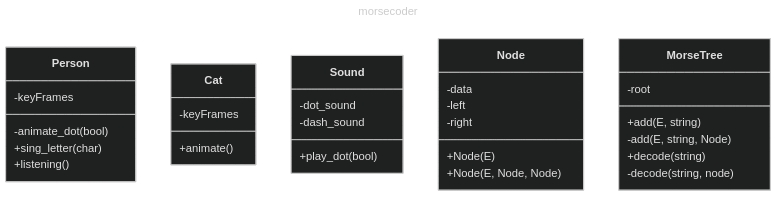
\includegraphics[scale=0.5]{o-1.png}
\end{center}

\begin{center}
    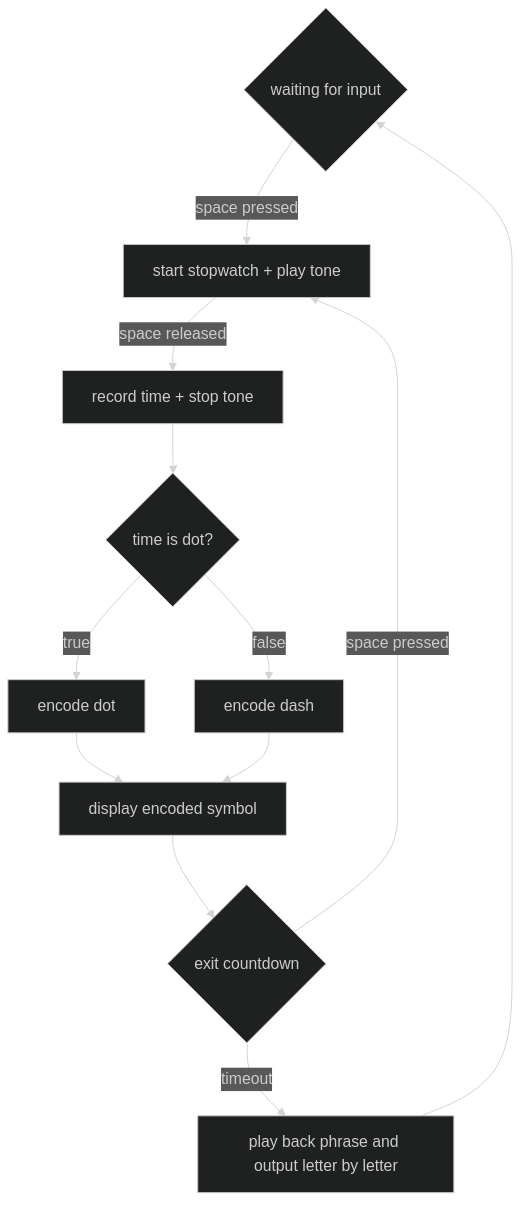
\includegraphics[scale=0.5]{o-2.png}
\end{center}

\end{document}
